% Tree of Life — a computational thesis.
% Build:  pdflatex main && bibtex main && pdflatex main && pdflatex main
% or:     latexmk -pdf main
\documentclass[11pt,a4paper]{article}

\usepackage[T1]{fontenc}
\usepackage[utf8]{inputenc}
\usepackage{lmodern}
\usepackage[margin=2.4cm]{geometry}
\usepackage{amsmath,amssymb,amsfonts}
\usepackage{booktabs}
\usepackage{graphicx}
\usepackage{xcolor}
\usepackage{tikz}
\usetikzlibrary{arrows.meta,positioning,shapes.geometric}
\usepackage[numbers,sort&compress]{natbib}
\usepackage[hidelinks]{hyperref}
\usepackage{caption}
\captionsetup{font=small,labelfont=bf}

\newcommand{\code}[1]{\texttt{\small #1}}
\newcommand{\SimStats}{\ensuremath{\mathrm{SimStats}}}
\DeclareMathOperator{\Var}{Var}
\DeclareMathOperator{\Cov}{Cov}
\DeclareMathOperator{\E}{\mathbb{E}}
\DeclareMathOperator{\KL}{D_{KL}}

\title{\textbf{Engineering Emergence}\\[2mm]
\large A Deterministic Instrument for the Physics of Open-Ended Evolution}
\author{Daven Ezhakieel}
\date{2026}

\begin{document}
\maketitle

\begin{abstract}
\noindent
Artificial-life systems generate open-ended phenomena but weak inference: a
striking run is a sample of one, mechanisms are entangled, and the vocabulary of
emergence admits no falsifier. Complex-systems theory has the opposite problem:
its accounts of criticality, critical slowing down, and open-ended evolution are
derived for low-dimensional or idealized models, and their domain of validity is
rarely tested against systems with genomes and selection.

This thesis joins the two. We specify a deterministic artificial ecology in
which every stochastic draw is keyed by $(\text{seed}, \text{tag}, t, \text{id})$,
the tick is a fixed ordered pipeline, and a rolling state hash fingerprints every
step; a TypeScript reference engine and a Rust/WebAssembly authority reproduce
each world \emph{bit-for-bit} from $(\text{seed}, \text{config})$. On that
substrate we build a measurement stack (documented observables, detectors, a
pre-registered claim ledger) and an experiment runner whose manifests are sha256
digests over the world fingerprint, trajectory, summary, and synthesis,
re-verified bit-for-bit.

We argue that determinism is not an engineering nicety but a \emph{causal
instrument}: it licenses branching the same history at the same tick with
exactly one intervention, so counterfactual and dose--response experiments
become available at a scale field ecology cannot reach. We use the instrument to
ask whether the generic theory of critical transitions \emph{transports} to an
evolving ecology. It does not, in a measurable way. Across 48 runs (8 seeds
$\times$ 6 ramp durations) and an 8-run no-ramp control, the ecology is
bistable and the control never collapses; variance is the only indicator
clearly above chance (pooled AUC $0.659$), flicker a distant second ($0.562$),
lag-1 autocorrelation and recovery at chance ($0.493$), and skewness
anti-predictive ($0.361$). The registered calibration prediction is
\emph{rejected}: warning skill declines monotonically with slower forcing
($0.72 \to 0.54$; slope $-0.0003$, $R^2 = 0.69$) and the lead in
control-parameter units shrinks (CV slope $-0.013$, $R^2 = 0.89$).

We treat the negative result as the scientific product and the instrument as
what makes it credible. We state the four candidate mechanisms (threshold drift,
detrending artifact, vanishing order parameter, evolutionary rescue), the
pre-registered multiverse and ablations that separate them, and a direct
impulse-response measurement of critical slowing down that the usual
autocorrelation proxy only approximates. The broader methodological claim is
that emergence claims should be adjudicated by a falsifier-first ledger with
artifact-level reproducibility, not by narrative or internal composite scores.
\end{abstract}

\section{Introduction}
Artificial-life (ALife) systems \citep{langton1990,ray1991,ofria2004} seek to
generate open-ended complexity from simple rules. Their scientific value,
however, is limited by inference: stochasticity, floating-point drift, and
undocumented mechanics make results hard to replicate and harder to compare, and
a rich run is usually a sample of one. Complex-systems research supplies the
missing standards --- order parameters, response functions, scaling, null
models --- but typically applies them to physical or low-dimensional systems.
The question this thesis pursues is whether those standards \emph{transport} to
a system with genomes, selection, and history.

\paragraph{Thesis.} A bit-deterministic artificial ecology is a \emph{causal
instrument}, not merely a simulator: because a world is a pure function of
$(\text{seed}, \text{config}, \text{intervention log})$, the same history can be
branched at any tick with one thing changed, and the divergence attributed to
that change. We use the instrument to test a specific, falsifiable proposition
from critical-transition theory --- that generic early-warning indicators give
calibrated notice of an approaching tipping point --- in a domain where the
theory's assumptions are violated by construction.

\paragraph{Contributions.}
\begin{enumerate}\setlength\itemsep{1pt}
\item a \textbf{deterministic instrument}: a dual-engine design (TypeScript
reference + Rust/WASM authority) with seeded streams, an ordered tick pipeline,
and bit-identical replay, plus a counterfactual protocol (branch, intervene,
measure);
\item a \textbf{measurement stack}: documented observables, detectors that emit
discrete claims, and a pre-registered scope ledger in which refutations are
results;
\item a \textbf{transport test} of early-warning theory in an evolving ecology,
including a registered rejection of the calibration prediction and an explicit
set of mechanisms that could explain it;
\item a \textbf{methodological claim}: emergence and open-endedness should be
adjudicated by falsifier-first ledgers and frozen analysis artifacts, not by
internal composite scores;
\item a \textbf{shared command layer} and dashboard that expose the same
experiment verbs in the browser and the console, so a replication is one
command away.
\end{enumerate}
Sections \ref{sec:related}--\ref{sec:disc} develop the system, its
mathematics, the registered questions, and the evidence.

\paragraph{What this is not.} The thesis does not claim to have demonstrated
open-ended evolution, nor that the critical-transition theory is false in
general. It claims that a specific, widely used family of indicators fails a
registered calibration test in a specific class of systems, and that the
failure is mechanistically tractable with the instrument described here.

\section{Related work}\label{sec:related}
\paragraph{Sciences of the artificial.} Simon argued that artificial systems are
legitimate scientific objects when their goals and mechanisms are specified
\citep{simon1962}; Holland framed emergence as constrained generation
\citep{holland1995}; Crutchfield recast structure as intrinsic computation
\citep{crutchfield1994}. Our thesis takes that programme literally: the
specification is the ordered tick pipeline, the measure is the observable
library, and the adjudication is a ledger.

\paragraph{Open-ended evolution.} Bedau's evolutionary activity statistics
\citep{bedau1998,bedau2003}, Fontana and Buss's organization of innovation
\citep{fontana1994}, and Taylor et al.'s operational criteria
\citep{taylor2016} define what it would mean for a system to keep producing
novelty; Kauffman's NK landscapes and the edge-of-chaos hypothesis
\citep{kauffman1993}, and Bak's self-organized criticality \citep{bak1987},
supply competing nulls. We use these as the standard against which our internal
ladders should eventually be judged, and we are explicit that we have not yet
met it.

\paragraph{Critical transitions.} The generic-indicator programme begins with
Scheffer et al. \citep{scheffer2009,scheffer2012} and the detection methodology of Dakos et
al. \citep{dakos2008,dakos2012}; empirical tests include Drake and Griffen's
extinction experiment \citep{drake2010} and Carpenter et al.'s whole-ecosystem
manipulation \citep{carpenter2011}. Limits and counterexamples are equally
important: Boettiger and Hastings on detectability \citep{boettiger2012},
Hastings and Wysham on warnings without warning \citep{hastings2010}, and Lenton
on climate tipping points \citep{lenton2011}. Our contribution is a transport
test in a system with genomes and selection, plus a direct response-function
measurement that the autocorrelation proxy only approximates.

\paragraph{Evolutionary and ecological theory.} Selection and transmission follow
Price \citep{price1970}; frequency-dependent dynamics follow the replicator
equation \citep{taylor1978}; major transitions in individuality
\citep{szathmary1995} motivate the open-endedness measurement; May's stability
criterion \citep{may1972} is the null against which claims of adaptive
complexity must be measured. Physiology, transport, and ecology use standard
models \citep{michaelis1913,berg1977,hodgkin1952,goldman1943,lindeman1942,holling1959}.
Complexity and information measures are classical
\citep{shannon1948,cover2006,lopezruiz1995,grassberger1983,lempelziv1976};
fractal geometry \citep{mandelbrot1982} and morphogenesis \citep{turing1952}
motivate the substrate. Statistical and reproducibility practice follows modern
norms \citep{student1908, welch1947,clopper1934,jeffreys1961,kass1995,nosek2018,steegen2016}.

\section{System architecture}\label{sec:arch}
The repository is a monorepo. A shared package holds types, the binary protocol,
and the terminal command layer; the \code{simulation} package holds the
TypeScript reference engine and the research lab; \code{crates/simulation} and
\code{crates/wasm} hold the Rust authority \citep{matsakis2014}; \code{apps/web} and
\code{apps/server} hold the dashboard and the HTTP/WS gateway.

\begin{figure}[t]\centering
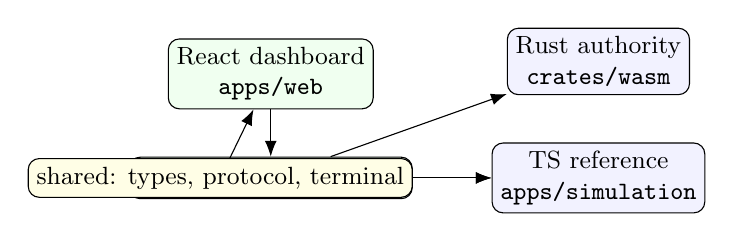
\begin{tikzpicture}[
  node distance=6mm and 10mm, >={Latex[length=2mm]},
  box/.style={draw,rounded corners,align=center,inner sep=3pt,font=\small},
  eng/.style={box,fill=blue!5}, web/.style={box,fill=green!6}, shr/.style={box,fill=yellow!10}]
\node[web] (ui) {React dashboard\\\code{apps/web}};
\node[web,below=of ui] (wk) {Worker / remote source};
\node[eng,right=of wk] (ts) {TS reference\\\code{apps/simulation}};
\node[eng,above=of ts] (wasm) {Rust authority\\\code{crates/wasm}};
\node[shr,left=of ts] (sh) {shared: types, protocol, terminal};
\draw[->] (ui) -- (wk);
\draw[->] (wk) -- (wasm);
\draw[->,dashed] (wk) -- (ts);
\draw[->] (sh) -- (ts);
\draw[->] (sh) -- (ui);
\end{tikzpicture}
\caption{Two engines behind one protocol; the terminal core is shared.}
\label{fig:arch}
\end{figure}

\section{The model and algorithms}\label{sec:model}
\paragraph{World.} Each world is a fractal escape-time field
$z \mapsto z^2 + c$ \citep{mandelbrot1982}; terrain properties (food, water,
chemistry, topology) are derived from the escape behaviour and the seed.

\paragraph{Agents.} An agent carries a genome (a fixed-length real vector; a
canonical size of 217 usable loci expanded to a 256-slot store), an energy and
water budget, a neural brain (Hebbian or back-propagation, optional POMDP
policy), and rich physiological state.

\paragraph{The tick.} One tick is a \emph{fixed ordered pipeline}. Order is part
of the specification: day/night and seasons $\to$ stochastic world $\to$ ecology
grounding $\to$ per agent (ascending id) a 23-stage chain (orbit, chem-terrain
sample, neighbour scan, pattern drives, movement, metabolism, water, feeding,
chemistry, DNA, omics, cells, immune, predator--prey, dormancy, reproductive
gene tracking, costly signalling, green-beard donation, memetic imitation,
reproduction, brain learning) $\to$ biome re-injection $\to$ replicator
projection (every 100 ticks) $\to$ fitness/births/events $\to$ mathematical and
biophysical observables $\to$ the world half (carrion, decomposition, plant
growth, weathering, signal diffusion, statistics).

\paragraph{Determinism.} Every stochastic path draws from a \code{SplitMix64}
stream keyed by $(\text{seed}, \text{tag}, t, \text{id})$; there is no global
randomness. A rolling FNV-1a \emph{state hash} $h_t$ fingerprints each tick and
underpins regression and parity tests.

\section{Mathematical foundations}\label{sec:math}
\paragraph{Drag fixed point.} With velocity update $v \leftarrow \alpha v +
F/m$ and clamping to $v_{\max}$, the terminal speed is
$v^\* = \min(v_{\max}, F/(m(1-\alpha)))$ for $\alpha \in (0,1)$.

\paragraph{Stochastic field.} An Ornstein--Uhlenbeck process
$dx = \theta(\mu - x)\,dt + \sigma\, dW$ has stationary variance
$\Var[x] = \sigma^2/(2\theta)$; Poisson burst pulses follow
$\Pr(k) = e^{-\lambda}\lambda^k/k!$.

\paragraph{Enzyme kinetics.} Substrate uptake follows Michaelis--Menten
$v = v_{\max}[S]/(K_m + [S])$ \citep{michaelis1913}.

\paragraph{Diffusion stability.} A 2-D explicit Laplacian update of a grid with
spacing $\Delta x$ and step $\Delta t$ is stable iff the diffusion number
$D\,\Delta t/\Delta x^2 \le \tfrac14$.

\paragraph{Learning.} TD(0) value updates $V(s) \leftarrow V(s) + \alpha[r +
\gamma V(s') - V(s)]$; Hebbian plasticity $\Delta w_{ij} = \eta\, a_i a_j$; and
back-propagation via the chain rule. Surprise is $|\delta|$ where
$\delta = r + \gamma V(s') - V(s)$.

\paragraph{Electrophysiology.} Membrane potential uses the Goldman--Hodgkin--Katz
relation \citep{hodgkin1952,goldman1943}
$V_m = \frac{RT}{F}\ln\frac{\sum P_i [i]_o}{\sum P_i [i]_i}$.

\paragraph{Ecology and selection.} Trophic transfer follows the 10\% rule
\citep{lindeman1942}; the replicator equation
$\dot{x}_i = x_i\big((Ax)_i - x^\top A x\big)$ \citep{taylor1978} is projected
every 100 ticks. The Price equation
$\Delta\bar{w} = \Cov(w,z)/\bar{w} + \E[w\,\Delta z]/\bar{w}$ \citep{price1970}
splits selection from transmission. Predation uses
$f(R) = aR/(1+ahR)$ \citep{holling1959}.

\paragraph{Diversity and complexity.} Shannon entropy
$H = -\sum p_i \log_2 p_i$ \citep{shannon1948}; Simpson
$1-\sum p_i^2$; LMC complexity $C = H \cdot D$ with
$D = \sum (p_i - 1/n)^2$ \citep{lopezruiz1995}; the Gini coefficient for energy
inequality; and the correlation dimension via Grassberger--Procaccia
\citep{grassberger1983}. Normalised mutual information between meme tags and
species is
$\mathrm{NMI} = I(X;Y)/\sqrt{H(X)H(Y)}$.

\paragraph{Dynamics.} The maximal Lyapunov exponent is estimated by
$\lambda = \lim_{t\to\infty}\tfrac1t \sum_t \ln|\delta z_t/\delta z_0|$
\citep{lyapunov1892,strogatz2018}; a Jacobi iteration solves the steady-state
field.

\paragraph{Statistics.} Welch's $t$-test \citep{welch1947}, Student's
$t$ \citep{student1908} via the incomplete beta function, Clopper--Pearson
intervals \citep{clopper1934}, one-way ANOVA, and Bayes factors with
Savage--Dickey--Raftery approximations \citep{jeffreys1961,kass1995}.

\section{Methodology}\label{sec:method}
\paragraph{Reproducibility.} A world is a fixpoint of $(\text{seed},
\text{config})$; trajectories are replayable. The experiment runner records a
manifest of sha256 digests (world fingerprint, trajectory, summary, synthesis);
\code{--verify} re-runs and compares bit-for-bit.

\paragraph{Objectives and search.} Emergence flags (L1--L3), adaptation,
steady-state, speciation, hazard/signal, and culture--species MI form a
multi-objective vector; search is random-with-elite, extensible to
hill-climbing and Pareto fronts.

\paragraph{Pre-registration.} Claims are registered before testing and resolved
with effect sizes and intervals, following reproducibility practice
\citep{nosek2018}. The ledger is append-only: a status may be revised only by
adding a dated entry that names the analysis that changed it. Composite
engineering scores (test counts, internal novelty heuristics) are reported as
quality assurance and are never treated as evidence for a scientific claim.

\paragraph{Counterfactual protocol.} The instrument's distinctive move is
branching: from a stored snapshot or an exact replay, run the same world twice
with one intervention applied to one branch, and measure the divergence in the
observables of interest. Because both branches share the seed and the
configuration, the difference is attributable to the intervention. Placebo
branches (an intervention with no modelled effect) bound the numerical and
scheduler noise.

\paragraph{Rare events.} Black-swan detectors (extinction, complexity collapse,
cooperation drop, culture loss) score impact and a surprise heuristic
$S = \text{impact}\,(1-p)/(p+\varepsilon)$, with joint probabilities bounded by
independence and Fr\'echet bounds.

\section{Research questions and the claim ledger}\label{sec:questions}
The programme is organized as questions with registered falsifiers rather than
as a narrative of findings. Table~\ref{tab:questions} reports the current
status; the open questions are the substance of the next phase.

\begin{table}[t]\centering
\caption{Registered questions. Status is as of this writing; \emph{open} means
the discriminating experiment has not yet been run.}\label{tab:questions}
\small
\begin{tabular}{p{0.7cm} p{5.6cm} p{4.4cm} p{2.6cm}}
\toprule
\# & Question & Registered falsifier & Status\\
\midrule
Q1 & Does at least one generic indicator separate pre-collapse from stationary
windows? & No indicator with AUC $> 0.5$ pooled over replicates & Supported\\
Q2 & Does variance out-rank autocorrelation-based indicators? & AR(1)/recovery
$\ge$ variance & Supported\\
Q3 & Is lead time calibrated in control-parameter units? & Lead in stress units
varies systematically with $\tau$ & Rejected\\
Q4 & Is the warning specific to the forcing? & No-ramp control collapses or
warns & Supported\\
Q5 & Is the Q3 failure threshold drift, detrending artifact, vanishing order
parameter, or evolutionary rescue? & A registered multiverse and ablation leave
the slope unexplained & Open\\
Q6 & Do spatial indicators transport where temporal ones fail? & Spatial AUC
$\le 0.5$ or no gain over temporal & Open\\
Q7 & Does a direct response-function measure succeed where AR(1) proxies fail? &
Perturbation recovery time does not rise before collapse & Open\\
Q8 & Does warning skill scale with system size? & AUC independent of $N$ across
100--2000 & Open\\
\bottomrule
\end{tabular}
\end{table}

\paragraph{Q5: four mechanisms.} The rejection of Q3 is phenomenological: it
establishes that calibration fails, not why. Four mechanisms are separable with
the existing instrument. \emph{M1 (threshold drift):} a slowly drifting baseline
widens the pre-ramp SD and raises the mean $+1.5$ SD bar; replace the baseline
with an EWMA or fix the threshold in stress units. \emph{M2 (detrending
artifact):} the 25-tick moving average removes the slow variance growth that is
the signal; run a multiverse over detrenders \citep{steegen2016}. \emph{M3
(vanishing order parameter):} extinction drives absolute variance to zero;
repeat with log population and with CV as the order parameter. \emph{M4
(evolutionary rescue):} selection on metabolic efficiency buffers the stress;
run a clonal, mutation-off ablation and measure genetic variance. A mechanism is
supported only if its manipulation removes at least half of the AUC--$\tau$
slope and the residual is not significant under a hierarchical bootstrap.

\paragraph{Q7: direct slowing-down.} Determinism permits the measurement the
AR(1) proxy approximates. At ticks along the ramp, branch the run, apply a
calibrated impulse (remove a fixed fraction of the population or inject a food
pulse), and measure the return time to the unperturbed trajectory; the recovery
rate $\lambda(t) = -\ln(\|\delta x(t+\Delta)\|/\|\delta x(t)\|)/\Delta$ is a
response function. Critical slowing down predicts $\lambda(t) \to 0$ before the
fold. If $\lambda(t)$ stays bounded while AUC falls, the proxy failure is a
property of the proxy, not evidence against slowing down.

\section{Results}\label{sec:results}
\begin{table}[t]\centering
\caption{Scope ledger, v1.0.0 (2026-10-16).}\label{tab:scope}
\begin{tabular}{l r}
\toprule
Outcome & Count\\
\midrule
Supported & 23\\
Refuted & 2\\
Inconclusive & 9\\
\midrule
Total & 34\\
\bottomrule
\end{tabular}
\end{table}

\begin{table}[t]\centering
\caption{Engineering verification. These are quality-assurance checks, not
scientific evidence, and are reported separately for that reason.}\label{tab:verify}
\begin{tabular}{l l}
\toprule
Check & Result\\
\midrule
Fast test tier & 45/45 files pass\\
Typecheck (shared, simulation, web) & clean\\
Cross-engine replay & bit-identical digests\\
Life-organization detector (internal) & rung O9 with all substrates enabled\\
\bottomrule
\end{tabular}
\end{table}

\paragraph{What the ledger teaches.} The two refuted claims are reported rather
than hidden: \textbf{C-AI-03} found the learned steerer \emph{worse} than a
do-nothing control, and \textbf{C-SIG-01}, a costly-signalling prediction, failed
in the tested regime. The first is a negative result about a plausible
intervention; the second is a boundary condition on a textbook prediction.
Neither is a failure of the platform. A ledger in which nothing is ever refuted
is a ledger that is not testing anything, and the engineering checks in
Table~\ref{tab:verify} are deliberately kept out of the evidence column.

\paragraph{Selection, not proof.} High-$N$ search identified several
high-complexity worlds (scores to 10.1), and the life-organization detector
reaches its ceiling only when all substrates are enabled. These are existence
proofs over a searched configuration space: they establish that the simulator
can produce the phenomenon, not that it does so for generic parameters. The
distinction matters for every claim in the ledger that rests on a selected
world.

\section{Critical transitions and early-warning signals}\label{sec:ews}
The project's focused vertical asks whether generic, model-free early-warning
indicators give calibrated advance notice of a macroscopic collapse. The
ecology is \emph{bistable} (a low state of $\approx 40$ agents and a high state
of $\approx 500$), and a no-ramp control survives in $8/8$ replicates. Ramping
metabolic load from $1$ to $40$ over a duration $\tau$ drives a reliable
collapse to extinction, so extinction is the critical transition and population
the order parameter. Indicators are computed on detrended rolling windows
(variance, lag-1 autocorrelation, recovery rate, coefficient of variation,
skewness, flickering) and scored by ROC area between pre-collapse and
early-stationary windows. The design is $8$ seeds $\times$ $6$ ramp durations
($\tau = 300,\dots,1050$ ticks), $48$ runs.

\begin{table}[t]\centering
\caption{Pooled early-warning skill over 43 collapsed runs (AUC; $0.5$ is
chance). Lead is measured in ticks and in control-parameter (metabolic-load)
units.}\label{tab:ews}
\begin{tabular}{l r r r}
\toprule
Indicator & AUC & Mean lead (ticks) & Mean lead (stress)\\
\midrule
Variance & 0.659 & 207 & 13.9\\
Flickering & 0.562 & 32 & 2.8\\
CV & 0.512 & 160 & 8.6\\
AR(1) / recovery & 0.493 & 39 & 1.4\\
Skewness & 0.361 & 50 & 3.9\\
\bottomrule
\end{tabular}
\end{table}

Variance is the workhorse indicator, flicker a distant second; the
autocorrelation-based indicators are at chance and skewness falls \emph{below}
chance. On this finer grid the AUC-vs-$\tau$ curve is \emph{monotone
decreasing} --- roughly $0.72$ for $\tau \le 750$ falling to $0.54$ for
$\tau \ge 900$ (slope $-0.0003$, $R^2 = 0.69$); the previously reported
``non-monotone'' curve was a four-replicate artefact. Consequently the
fixed distance-to-bifurcation prediction is rejected: the lead measured in
stress units \emph{shrinks} with $\tau$ (CV slope $-0.013$, $R^2 = 0.89$) rather
than staying constant, so warning quality degrades as the tipping point is
approached more slowly. The experiment is fully reproducible via
\texttt{npm run research:ews}.

\paragraph{What this licenses, and what it does not.} It licenses the statement
that, under this registered analysis in this ecology, the autocorrelation family
carries no warning and calibration fails. It does not identify why, and with
eight seeds per cell the confidence interval on a mean AUC is wide (order
$\pm 0.1$); the detection rule is one choice among many, and windows within a
run are not independent. These are not caveats appended after the fact: they are
the reason Q5 is registered as open, with a multiverse and ablations rather than
a narrative, and the reason the next phase increases replicates before it
increases claims.

\section{Discussion}\label{sec:disc}
\paragraph{What the instrument changes.} Treating emergence as an engineering
objective forces (a) determinism and parity, (b) explicit objectives and
thresholds, (c) multi-seed aggregation to avoid single-seed overfitting, and (d)
re-runnable records. But the deeper change is epistemic: once a world is a pure
function of its inputs, a \emph{negative} result becomes cheap. If variance is the
only indicator that works, the obvious objection --- ``you ran a different
system'' or ``the run drifted'' --- is answered by the digest, not by argument.
That is what lets a simulator contribute to theory rather than merely illustrate
it.

\paragraph{Threats to validity.}
\emph{Construct:} AUC is not lead time, and extinction is not a fold
bifurcation; a ramped die-off may be a transcritical or saddle-node crossing, and
the theory's predictions differ. \emph{Internal:} the detection threshold is
estimated from the pre-ramp plateau, which a slow ramp inflates (M1), and the
detrender removes slow variance (M2); both are testable and currently untested.
\emph{External:} one ecology, one genotype--phenotype map, one topology, one
noise model --- the claim is about this class of systems until replicated.
\emph{Statistical:} eight seeds per cell, non-independent windows within a run,
and a multiple-comparison surface of five indicators by six ramp lengths.
\emph{Conclusion:} the mechanism is unidentified; ``the theory does not
transport'' is supported, ``because of adaptation'' is not.

\paragraph{What would falsify the thesis.} T1 fails if replay is not exact under
interventions, or if counterfactual divergence is dominated by floating-point or
scheduler effects. T2 collapses to a methods caveat if a pre-registered
multiverse shows the AUC--$\tau$ slope is an artifact of the threshold rule or
the detrender and vanishes under every reasonable specification. T3 fails if
ledger statuses can be revised after seeing the data without recording the
revision. Each failure mode is named here so that the next phase can be judged
against it.

\paragraph{Programme.} Three papers, in order. \emph{A (instrument):}
deterministic replay as a causal instrument for artificial life ---
specification, parity, manifests, counterfactual protocol. \emph{B (negative
result and mechanism):} ``Generic early-warning signals do not transport to an
evolving ecology: a registered multiverse and ablation'', with Q5--Q8 as the
registered extension. \emph{C (open-endedness):} a falsifier-first ledger for
open-ended evolution, using evolutionary activity \citep{bedau1998,bedau2003},
novelty, and a major-transition detector \citep{szathmary1995}, each with a null.
The immediate sequence is to freeze the present analysis as the registered
baseline, run Q5 with 32--64 seeds, run Q7's impulse response, and only then
extend to substrates and topologies.

\begin{table}[t]\centering
\caption{Gap analysis for a programme-level contribution. Each row is
actionable with the existing instrument; determinism is what makes rows three
through six feasible at all.}\label{tab:programme}
\small
\begin{tabular}{p{2.6cm} p{5.4cm} p{5.0cm}}
\toprule
Requirement & Current state & Next artifact\\
\midrule
Theory & Verbal expectation of critical slowing down & Derive AUC($\tau$) for
a ramped fold with demographic noise\\
Mechanism & Q3 rejection is phenomenological & Q5 multiverse + M1--M4
ablations\\
Causal identification & Determinism and replay implemented & Q7
impulse-response; placebo ramps; dose--response\\
Scaling & Single $N \approx 300$--$500$ & Q8 finite-size sweep, 100--2000\\
Generalization & One ecology and topology & Substrate and topology
replication\\
Statistics & 8 seeds, one analysis path & 32--64 seeds; hierarchical bootstrap;
multiverse\\
Open-endedness & Internal ladder O0--O9 & Bedau activity, novelty rate,
major-transition detector\\
Artifacts & Digests, manifests, dashboard & Frozen analysis code; archived
manifests; one-command replication\\
\bottomrule
\end{tabular}
\end{table}

\paragraph{Limitations of the substrate.} The opt-in omics/quantum layers
(E--J) are \emph{readings of shared pools}; the TypeScript reference reports
zeros there by design, so their numbers are WASM-only and should not be pooled
across engines. A ``supported'' verdict is statistical, not proof; the ledger's
intervals are the relevant statement. Current search is random-with-elite rather
than a full Pareto campaign, so the high-complexity worlds reported in the
research outputs are existence proofs over a sampled space, not typical outcomes.

\section{Conclusion}\label{sec:concl}
Tree of Life shows that a rich artificial-life substrate can be made
deterministic, measurable, and experimentable without sacrificing depth --- and,
more importantly, that determinism changes what the substrate can be used
\emph{for}. The early-warning study is the proof of concept: a theory imported
from dynamical systems was given a fair test, failed its calibration prediction
in a measurable way, and left a tractable set of mechanisms rather than a
rhetorical dispute. The two refutations already in the ledger are the same
phenomenon at smaller scale: a laboratory that cannot lose is not measuring
anything. The next step is not a larger simulator but a sharper instrument ---
frozen analyses, more replicates, direct response functions, and a ledger that
keeps score.

\bibliographystyle{plainnat}
\bibliography{references}

\end{document}
